
\chapter{Solar wind impact on the terrestrial magnetosphere}

% Alle Presis ausschlachten!
% Alle Projektberichte ausschlachten!
% Kp8--Liste irgendwo einweben...
% paper draft 2014 ausschlachten... Check!

%Questions addressed in this thesis
Questions:\\
	How strong is the solar wind influence on the terrestrial magnetosphere?\\
	How strong do different structure types influence the terrestrial magnetosphere?\\
	
	How can the impact strength of the solar wind be forecasted? (VBz->Kp L1-Alerts)\\
	How can the impact strength of CMEs be forecasted (V->Kp correlation for CMEs)?\\
	(How can the impact field strength of CMEs be forecasted (V->B correlation for CMEs)?)\\

On solar wind acceleration and SPP proposition: McComas2007\\

% Analyses structure:\\
% 
% Core studies:
% Motivational question: Which solar wind structures contribute to the individual Kp ranges?
% define OMNI data set duration
% build Kp histogram
% 	for each Kp range
% 		extract contributing solar wind sections
% 			get sections structure flag
% 		derive individual structure contribution
% 
% preparations:
% analyze solar wind and categorize its structure types
% 	define thresholds for event recognition
% 	write automatic event recognition program
% 	=> flagged time series
% 	(additional output: OMNI solar wind event list)
% 
% applications:
% - Kp nowcast with L1 solar wind measurements (L1 alerts, disseminated as RSS feeds; integrated in smartphone app and space weather display)
% - Forecast of the possible CME impact on the Earths magnetosphere (Kp index) from the predicted CME arrival velocity (integrated in UGOE CME forecast chain (aka DDC))
% 
% 
% Further studies:
% Motivational question: What is the evolution of the solar wind parameters/structures before arriving at Earth? %what is meant by the term evolution?
% define Helios data set
% extrapolation of the solar wind parameters with the use of regression fitting
% extraction of distance independent time series with regression fits
% get flagged time series from distance independent time series
% (like before:)
% analyze solar wind and categorize its structure types
% 	define thresholds for event recognition
% 	write automatic event recognition program
% 	=> flagged time series
% 	(additional output: Helios solar wind event list)
% 
% 
% empirical radial solar wind model:
% derive the characteristic distributions of the solar wind parameters from OMNI data
% combination of the OMNI characteristic distributions with the Helios extrapolation
% 	(additional output: empirical radial probability distribution model)
% 
% Applications:
% - The near-sun* solar wind extrapolation can be useful for the planned Solar Probe Plus mission


\section{Quantifying solar wind impact on the terrestrial magnetosphere}

linear velocity replacement of ACE realtime data with Kp, Machol2013\\

3hmin(vBzgsm) performs in rank correlation slightly better than the sophisticated Newell formula\\

choosing solar wind parameters\\
	comparison of their correlation coefficients in table...\\
		-> Pearson or Spearman rank cc?? (Appendix?)\\
		-> lag meaning?\\
	% bulk correlation coefficients and functions\\
	% B-Kp, V-Kp, Bz-Kp
	
What kind of correlation function with these parameters?\\
% comparison with existing solar wind-magnetosphere coupling functions (see Basics chapter)\\

comparison of correlation coefficients for different data resolutions and measures in \autoref{tab:cc_measure_comparison}.
\begin{table}[htb]\small
	\centering
	\captionsetup{belowskip=4pt}
	\caption{Pearson correlation coefficients of Kp with sample solar wind parameters for different data resolutions and measures for comparison. 3h 1min extrema data results in slightly higher ccs... (use Spearman instead?)}
	\begin{tabular}{lcccc}
		\toprule
			&OMNI 1h	&OMNI 1h	&OMNI 1min	&OMNI 1min\\
			&1963-201308	&1963-201308	&19850101-20150101	&19850101-20150101\\
			&3h mean	&3h 1h extrema	&3h 10min extrema	&3h 1min extrema\\
		\midrule
		V	&0.568	&0.579	&?	&0.598\\
		B	&	&	&	&\\
		\bottomrule
	\end{tabular}
	\label{tab:cc_measure_comparison}
\end{table}


correlation coefficients in \autoref{tab:correlation_coefficients}.
\begin{table}[htb]\small
	\centering
	\captionsetup{belowskip=4pt}
	\caption{Pearson correlation coefficients of Kp with solar wind parameters... (use Spearman instead?)}
	\begin{tabular}{cc}
		\toprule
			&OMNI 1min\\
		Parameter	&19850101-20150101\\
			&3h 1min max\\
		\midrule
		N	&0.199792\\
		V	&0.598351\\
		T	&0.510607\\
		B	&0.595860\\
		Bzgsm	&-0.666050$^\text{a}$\\
		V*B	&0.682383\\
		V*Bzgsm	&-0.715101$^\text{a}$\\
		N*T	&\\
		\bottomrule
		\multicolumn{2}{l}{\footnotesize{$^\text{a}$Here it is min instead of max.}}
	\end{tabular}
	\label{tab:correlation_coefficients}
\end{table}


Results of this section\\
What kind of solar wind structures create the individual regions in this distribution? -> next section\\
What is their individual contribution to the Kp ranges (e.g. high Kp: CMEs 70\% and CIRs 30\%)? -> next section\\

maybe correlation coefficient frequency spectra over time...?\\


\section{Solar wind structure type influence on the terrestrial magnetosphere}

Kp vs VBzgsm - CMEs as fraction of overall solar wind; see \autoref{fig:OMNI_HRO_1MIN_19810101-20130731_with_ap_vBzgsm_3hmin_CMEpart_VBzgsmvsKp_2Dhistogram_plot}
\begin{figure}[htb]
	\centering
	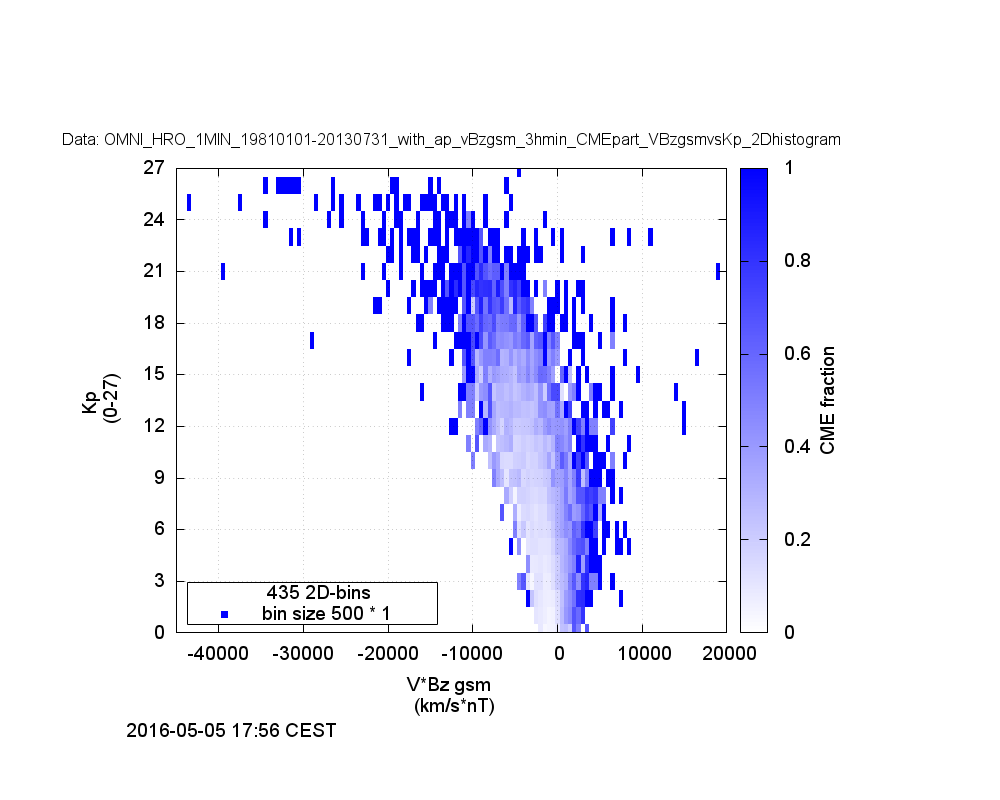
\includegraphics[width=0.3\textwidth]{images/gnuplots/OMNI_HRO_1MIN_19810101-20130731_with_ap_vBzgsm_3hmin_CMEpart_VBzgsmvsKp_2Dhistogram_plot.png}
	\caption{CMEs as fraction of overall solar wind. sws1/sws}
	\label{fig:OMNI_HRO_1MIN_19810101-20130731_with_ap_vBzgsm_3hmin_CMEpart_VBzgsmvsKp_2Dhistogram_plot}
\end{figure}

\subsection{Solar wind seasonal dependence}
seasonal variation by month\\
quantify variation amplitudes\\

see \autoref{fig:OMNI_monthly_freq_V_gps}
\begin{figure}[htb]
	\centering
	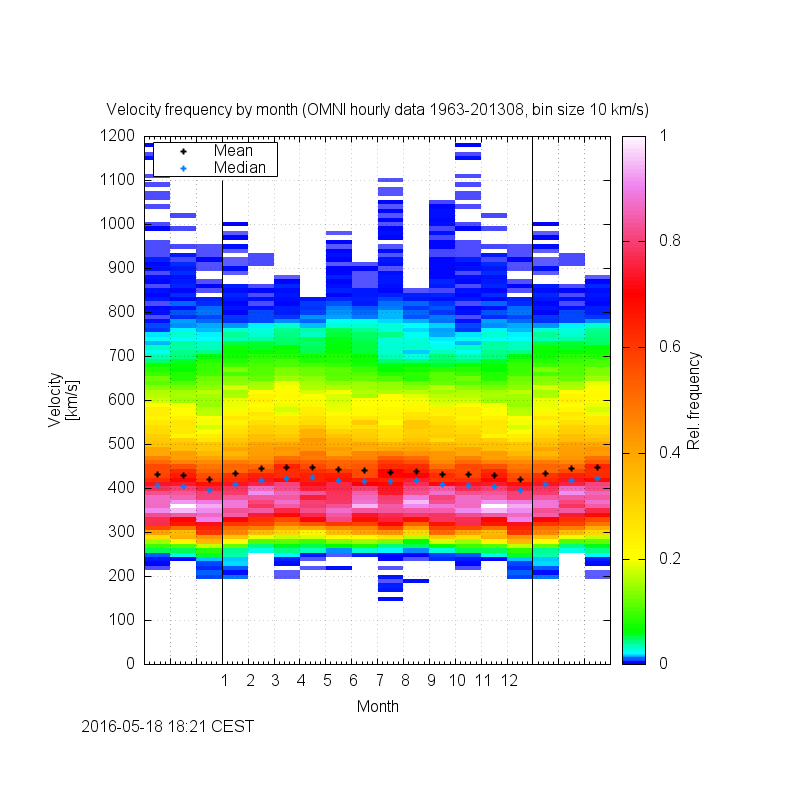
\includegraphics[width=0.3\textwidth]{images/gnuplots/OMNI_monthly_freq_V_gps.png}
	\caption{Diagram of the velocity frequency by month for the period 1963/01--2013/08. Mean and median values are shown as well.}
	\label{fig:OMNI_monthly_freq_V_gps}
\end{figure}

derived exponent values from simple trigonometric fit on monthly values:\\
$c_N = -2.234$\\
maybe figure?\\

...following maybe into section 'radial dependence of median value?\\
expected influence from perihelion/aphelion (see Appendix...) distance vs observations\\
we expect for the proton density (scaling law $N(r) = 7.6~\text{cm}^{-3} \cdot r^{-2}$):\\
N(0.983~au) = 7.9~cm$^{-3}$\\
N(1~au) = 7.6~cm$^{-3}$\\
N(1.017~au) = 7.3~cm$^{-3}$\\
we expect for the magnetic field strength (scaling law $\propto r^{-1.6}$):\\
B(0.983~au) = 6.3~nT\\
B(1~au) = 6.1~nT\\
B(1.017~au) = 5.9~nT\\

see \autoref{fig:OMNI_monthly_freq_B_a_gps}
\begin{figure}[htb]
	\centering
	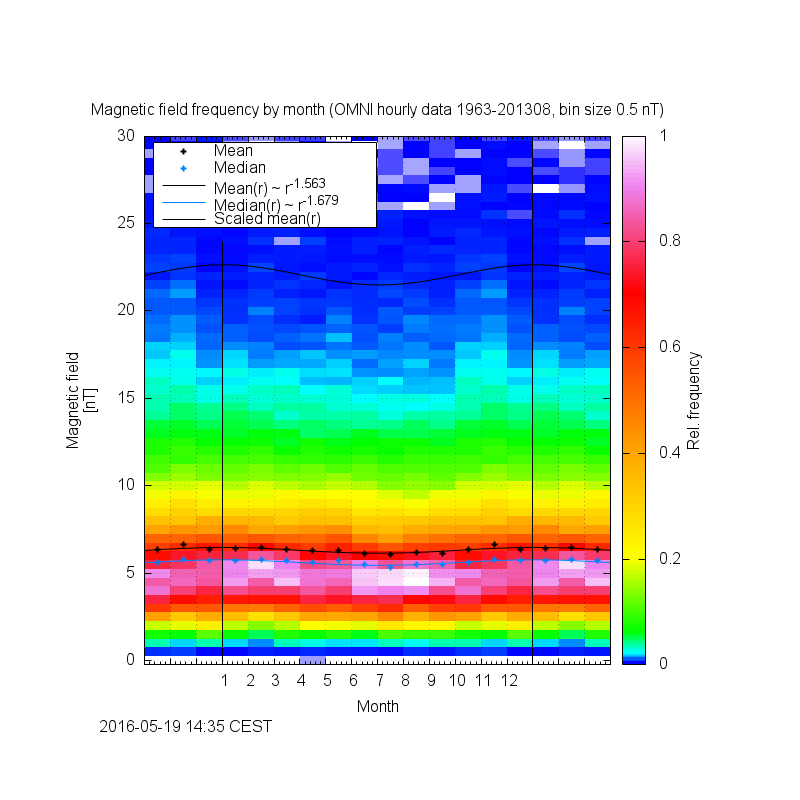
\includegraphics[width=0.3\textwidth]{images/gnuplots/OMNI_monthly_freq_B_a_gps.png}
	\caption{Diagram of magnetic field frequency by month for the period 1963/01--2013/08. Mean and median values are shown as well as the expected course from the solar distance variation (obtained from Helios data).}
	\label{fig:OMNI_monthly_freq_B_a_gps}
\end{figure}

\section{Kp solar cycle dependence}
- solar cycle variations\\
- variations between solar cycles\\

the yearly Kp frequency shows variations; the yearly mean Kp shifts about 2~units.\\
plot of the yearly Kp frequency (see \autoref{fig:Kp_freq_yearly_ssn_plot})
\begin{figure}[htb]
	\centering
	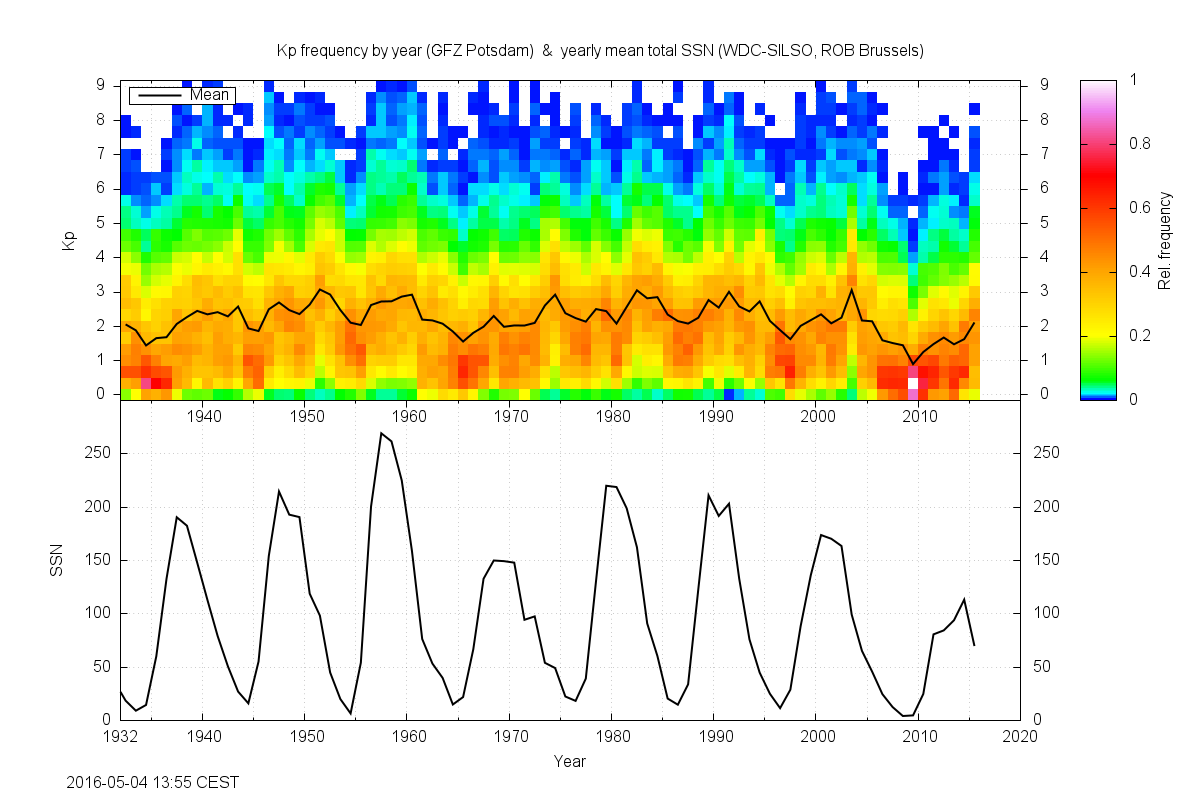
\includegraphics[width=0.3\textwidth]{images/gnuplots/Kp_freq_yearly_ssn_plot.png}
	\caption{Kp frequency by year, yearly mean Kp and yearly mean total SSN for the years 1932--2015. The pattern of Kp shows an imprint of the solar cycle. Kp data from GFZ German Research Centre for Geosciences, Potsdam, Germany and SSN data from WDC-SILSO, Royal Observatory of Belgium, Brussels.}
	\label{fig:Kp_freq_yearly_ssn_plot}
\end{figure}
add Kp--SSN matrix plot...\\

analyze Kp frequency by month for different SWSs\\
analyze Kp frequency by year for different SWSs\\
put into later part of analysis...

\subsection{Kp seasonal dependence}
for high Kp values (>~4?) there are yearly frequency maxima at the equinoxes and minima at the solstices. this variation amounts to more than 1~Kp (see figure...)

possible causes (see \citet{Rangarajan1997} p. 1282 and mention Bartels1963 too):\\
- Earth's rotation axis tilt ($\pm23.44$\textdegree) (obliquity to orbit/inclination of equator)\\
- solar rotation axis tilt ($\pm7.25$\textdegree) (cite 'NASA Earth fact sheet')\\
- varying distance from Sun 0.983--1.0167~au ($\pm3.3~\%$)\\
- changing solar cycle polarity gives two superimposed maxima... -> No. see even/odd plots\\

read Bothmer1998 Ch 3...\\


\section{Summary/Results}
sw-nowcast: vBzgsm-Kp relation (average and worst case)\\
CME-forecast: v-Kp relation (average and worst case)\\

seasonal correction: $\Delta$Kp(month)\\
$Kp_\text{impact} = Kp_\text{CME} \pm \Delta Kp(month)$\\

sw-timeseries ACE OPTIMAP ``Zeitreihe''-events

\section{Forecast}

\subsection{Internal solar wind correlations}
B-V correlation\\
ACE MAGSWE 64~s data -> yearly overlay plot\\

\section{Applications}
rssfeeds, rtsw plots\\
CME Kp impact\\
part of DDC\\

